% \documentclass[tikz]{standalone}
% \usepackage{tikz}
% \usetikzlibrary{decorations.pathreplacing}
% \begin{document}
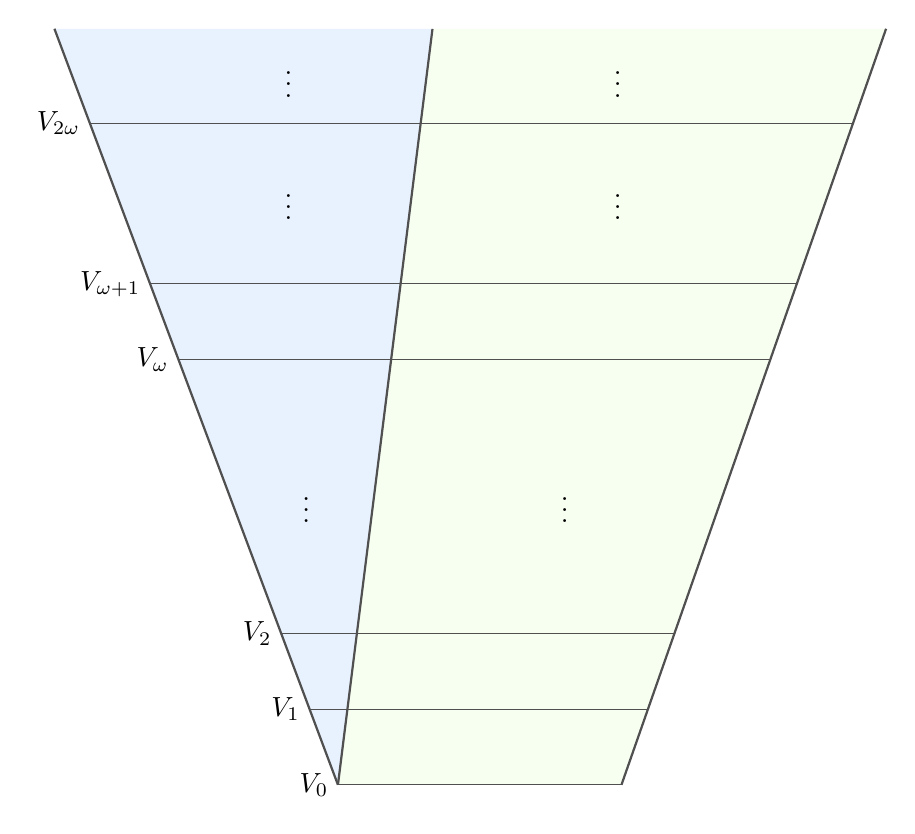
\begin{tikzpicture}[scale=1.2]
    % Define colors
    \definecolor{purecolor}{RGB}{210, 230, 255}
    \definecolor{impurecolor}{RGB}{230, 255, 210}
    \definecolor{linecolor}{RGB}{80, 80, 80}

    % Define the straight boundary points
    \coordinate (bottomL) at (-3, 0);
    \coordinate (topL) at (-6, 8);
    \coordinate (bottomR) at (0, 0);
    \coordinate (topR) at (2.8, 8);

    % Define y-coordinates for each level
    \def\yV{0}
    \def\yI{0.8}
    \def\yII{1.6}
    \def\ydots{3}
    \def\yomega{4.5}
    \def\yomegaplus{5.3}
    \def\ydotstwo{6.5}
    \def\ytwoomega{7}

    % Calculate x-coordinates on the straight boundaries for each level
    % Left boundary: interpolate between (-3,0) and (-6,8)
    \coordinate (V0L) at ({-3 + (-3) * \yV / 8}, \yV);
    \coordinate (V1L) at ({-3 + (-3) * \yI / 8}, \yI);
    \coordinate (V2L) at ({-3 + (-3) * \yII / 8}, \yII);
    \coordinate (VdL) at ({-3 + (-3) * \ydots / 8}, \ydots);
    \coordinate (VwL) at ({-3 + (-3) * \yomega / 8}, \yomega);
    \coordinate (Vw1L) at ({-3 + (-3) * \yomegaplus / 8}, \yomegaplus);
    \coordinate (Vd2L) at ({-3 + (-3) * \ydotstwo / 8}, \ydotstwo);
    \coordinate (V2wL) at ({-3 + (-3) * \ytwoomega / 8}, \ytwoomega);

    % Right boundary: interpolate between (0,0) and (2.8,8)
    \coordinate (V0R) at ({0 + 2.8 * \yV / 8}, \yV);
    \coordinate (V1R) at ({0 + 2.8 * \yI / 8}, \yI);
    \coordinate (V2R) at ({0 + 2.8 * \yII / 8}, \yII);
    \coordinate (VdR) at ({0 + 2.8 * \ydots / 8}, \ydots);
    \coordinate (VwR) at ({0 + 2.8 * \yomega / 8}, \yomega);
    \coordinate (Vw1R) at ({0 + 2.8 * \yomegaplus / 8}, \yomegaplus);
    \coordinate (Vd2R) at ({0 + 2.8 * \ydotstwo / 8}, \ydotstwo);
    \coordinate (V2wR) at ({0 + 2.8 * \ytwoomega / 8}, \ytwoomega);

    % Fill the impure hierarchy (total area minus pure triangle)
    \fill[impurecolor, opacity=0.3] (bottomL) -- (bottomR) -- (topR) -- (-2, 8) -- cycle;

    % Fill the pure hierarchy (triangular part with tip at bottom left)
    \fill[purecolor, opacity=0.5] (bottomL) -- (-2, 8) -- (topL) -- cycle;

    % Draw the straight boundary lines
    \draw[thick, linecolor] (bottomL) -- (topL);
    \draw[thick, linecolor] (bottomR) -- (topR);

    % Draw horizontal level lines (only for labeled stages)
    \draw[linecolor] (V0L) -- (V0R);
    \draw[linecolor] (V1L) -- (V1R);
    \draw[linecolor] (V2L) -- (V2R);
    \draw[linecolor] (VwL) -- (VwR);
    \draw[linecolor] (Vw1L) -- (Vw1R);
    \draw[linecolor] (V2wL) -- (V2wR);

    % Draw the pure hierarchy boundary (diagonal from bottom left tip)
    \draw[thick, linecolor] (bottomL) -- (-2, 8);

    % Add level labels on the left
    \node[left] at (V0L) {$V_0$};
    \node[left] at (V1L) {$V_1$};
    \node[left] at (V2L) {$V_2$};
    \node[left] at (VwL) {$V_\omega$};
    \node[left] at (Vw1L) {$V_{\omega+1}$};
    \node[left] at (V2wL) {$V_{2\omega}$};

    % Add dots for skipped stages (inside the hierarchy)
    \node at ({-3 + (-3) * 2.5 / 8 + 0.6}, 3) {$\vdots$};
    \node at ({-3 + (-3) * 3 / 8 + 0.6}, 6.2) {$\vdots$};
    \node at ({-3 + (-3) * 3 / 8 + 0.6}, 7.5) {$\vdots$};

    % Add dots on the right side too (inside the hierarchy)
    \node at ({0 + 2.8 * 0 / 8 - 0.6}, 3) {$\vdots$};
    \node at ({0 + 2.8 * 1.6 / 8 - 0.6}, 6.2) {$\vdots$};
    \node at ({0 + 2.8 * 1.6 / 8 - 0.6}, 7.5) {$\vdots$};

\end{tikzpicture}
% \end{document}
